% !TEX encoding = UTF-8 Unicode

%
% Exemple de rapport
% par Pierre Tremblay, Universite Laval
% modifié par Christian Gagne, Universite Laval
% modifié par Francis Valois, Université Laval
% 31/01/2011 - version 1.4
%

%
% Modele d'organisation d'un projet LaTeX 
% rapport/      dossier racine et fichier principal
% rapport/fig   fichiers des figures
% rapport/tex   autres fichiers .tex
%

% ** Preambule **
%
% Ajouter les options au besoin :
%    - "ULlof" pour inclure la liste des figures, requis si "\begin{figure}" utilise
%    - "ULlot" pour inclure la liste des tableaux, requis si "\begin{table}" utilise
%
\documentclass[12pt,ULlof,ULlot]{ULrapport}

% Chargement des packages supplementaires (si absent de la classe)
\usepackage[utf8]{inputenc}
\usepackage[T1]{fontenc}
\usepackage[autolanguage]{numprint}
\usepackage{icomma}
\usepackage{subfigure}
\usepackage{graphicx}
\usepackage[absolute]{textpos}
\usepackage[final]{pdfpages}
\usepackage{listings} % For source code
\usepackage{color}
\usepackage{pdflscape}
\usepackage{multirow}
\usepackage{array}

% settings pour le listing de code
\lstset{
	tabsize=4,
	language=matlab,
        basicstyle=\scriptsize,
        %upquote=true,
        aboveskip={1.5\baselineskip},
        columns=fixed,
        showstringspaces=false,
        extendedchars=true,
        breaklines=true,
        prebreak = \raisebox{0ex}[0ex][0ex]{\ensuremath{\hookleftarrow}},
	frame=single,
        showtabs=false,
        showspaces=false,
        showstringspaces=false,
        identifierstyle=\ttfamily,
        keywordstyle=\color[rgb]{0,0,1},
        commentstyle=\color[rgb]{0.133,0.545,0.133},
        stringstyle=\color[rgb]{0.627,0.126,0.941},
	language=Java
}
\newcommand{\HRule}{\rule{\linewidth}{0.2mm}}
%\usepackage[hmargin=3cm,vmargin=3.5cm]{geometry}
\definecolor{mygrey}{gray}{.96} % Light Grey
\lstset{ 
	language=vhdl,              % choose the language of the code
%("language=Verilog" is popular as well)
	tabsize=4,			% sets the size of the tabs in spaces (1
%Tab is replaced with 3 spaces)
	basicstyle=\scriptsize,               % the size of the fonts that are
%used for the code
	numbers=left,                   % where to put the line-numbers
	numberstyle=\tiny,              % the size of the fonts that are used
%for the line-numbers
	stepnumber=1,                   % the step between two line-numbers. If
%it's 1 each line will be numbered
	numbersep=5pt,                  % how far the line-numbers are from the
%code
	backgroundcolor=\color{mygrey}, % choose the background color. You must add \usepackage{color}
	showspaces=false,              % show spaces adding particular underscores
	showstringspaces=false,        % underline spaces within strings
	%showtabs=false,                % show tabs within strings adding particular underscores
	frame=single,	                 % adds a frame around the code
	tabsize=3,	                    % sets default tabsize to 2 spaces
	captionpos=b,                   % sets the caption-position to bottom
	breaklines=true,                % sets automatic line breaking
	breakatwhitespace=false,        % sets if automatic breaks should only happen at whitespace
	%escapeinside={\%*}{*)},        % if you want to add a comment within your code
	%commentstyle=\color{RedBrick}   % sets the comment style
}

\def\dbar{{\mathchar'26\mkern-12mu d}} 
%\usepackage[options]{nom_du_package}

% Definition d'une commande pour presenter des cellules multilignes dans un tableau
\newcommand{\cellulemultiligne}[1]{\begin{tabular}{@{}c@{}}#1\end{tabular}}


% Definition de colonnes en mode paragraphe avec alignement ajustable
% Cette definition requiert le chargement du package "array"
%    - alignement horizontal, parametre #1 : - \raggedright (aligne a gauche)
%                                            - \centering (centre)
%                                            - \raggedleft (aligne a droite)
%    - alignement vertical, parametre #2 : - p (aligne en haut)
%                                          - m (centre)
%                                          - b (aligne en bas)
%    - largeur, parametre #3 : longueur
\newcolumntype{Z}[3]{>{#1\hspace{0pt}\arraybackslash}#2{#3}}

% Definitions des parametres de la page titre
\TitreProjet{Livrable 4 - Robot Kinocto}                         % Titre du projet
\TitreRapport{Design III}       % Titre du rapport
\Destinataire{M. Dominique Grenier, M. Luc Lamontagne et M. Abdelhakim Bendada}         % Nom(s) du destinataire
\TableauMembres{%                                     % Tableau des membres de l'equipe
   910\,058\,073  & Émile Arsenault \\\hline 
   908\,190\,985  & Philippe Bourdages \\\hline
   910\,098\,468  & Pierre-Luc Buhler \\\hline    
   998\,107\,355  & Diane Fournier \\\hline
   908\,318\,388  & Olivier Sylvain \\\hline
   910\,055\,897  & Daniel Thibodeau \\\hline
   910\,097\,879  & Francis Valois \\\hline
}
\DateRemise{21 avril 2013}                           % Date de remis


% Corps du document

\begin{document}

%   Chapitres

%!TEX root = ../rapport.tex
%!TEX encoding = UTF-8 Unicode

% Chapitres "Introduction"

% modifié par Francis Valois, Université Laval
% 31/01/2011 - version 1.0 - Création du document

\chapter{Matrice de vérification des performances}
%\label{s:sequences}
Ce chapitre présente la matrice de vérification des performances
%\begin{figure}[htb]
%\centering
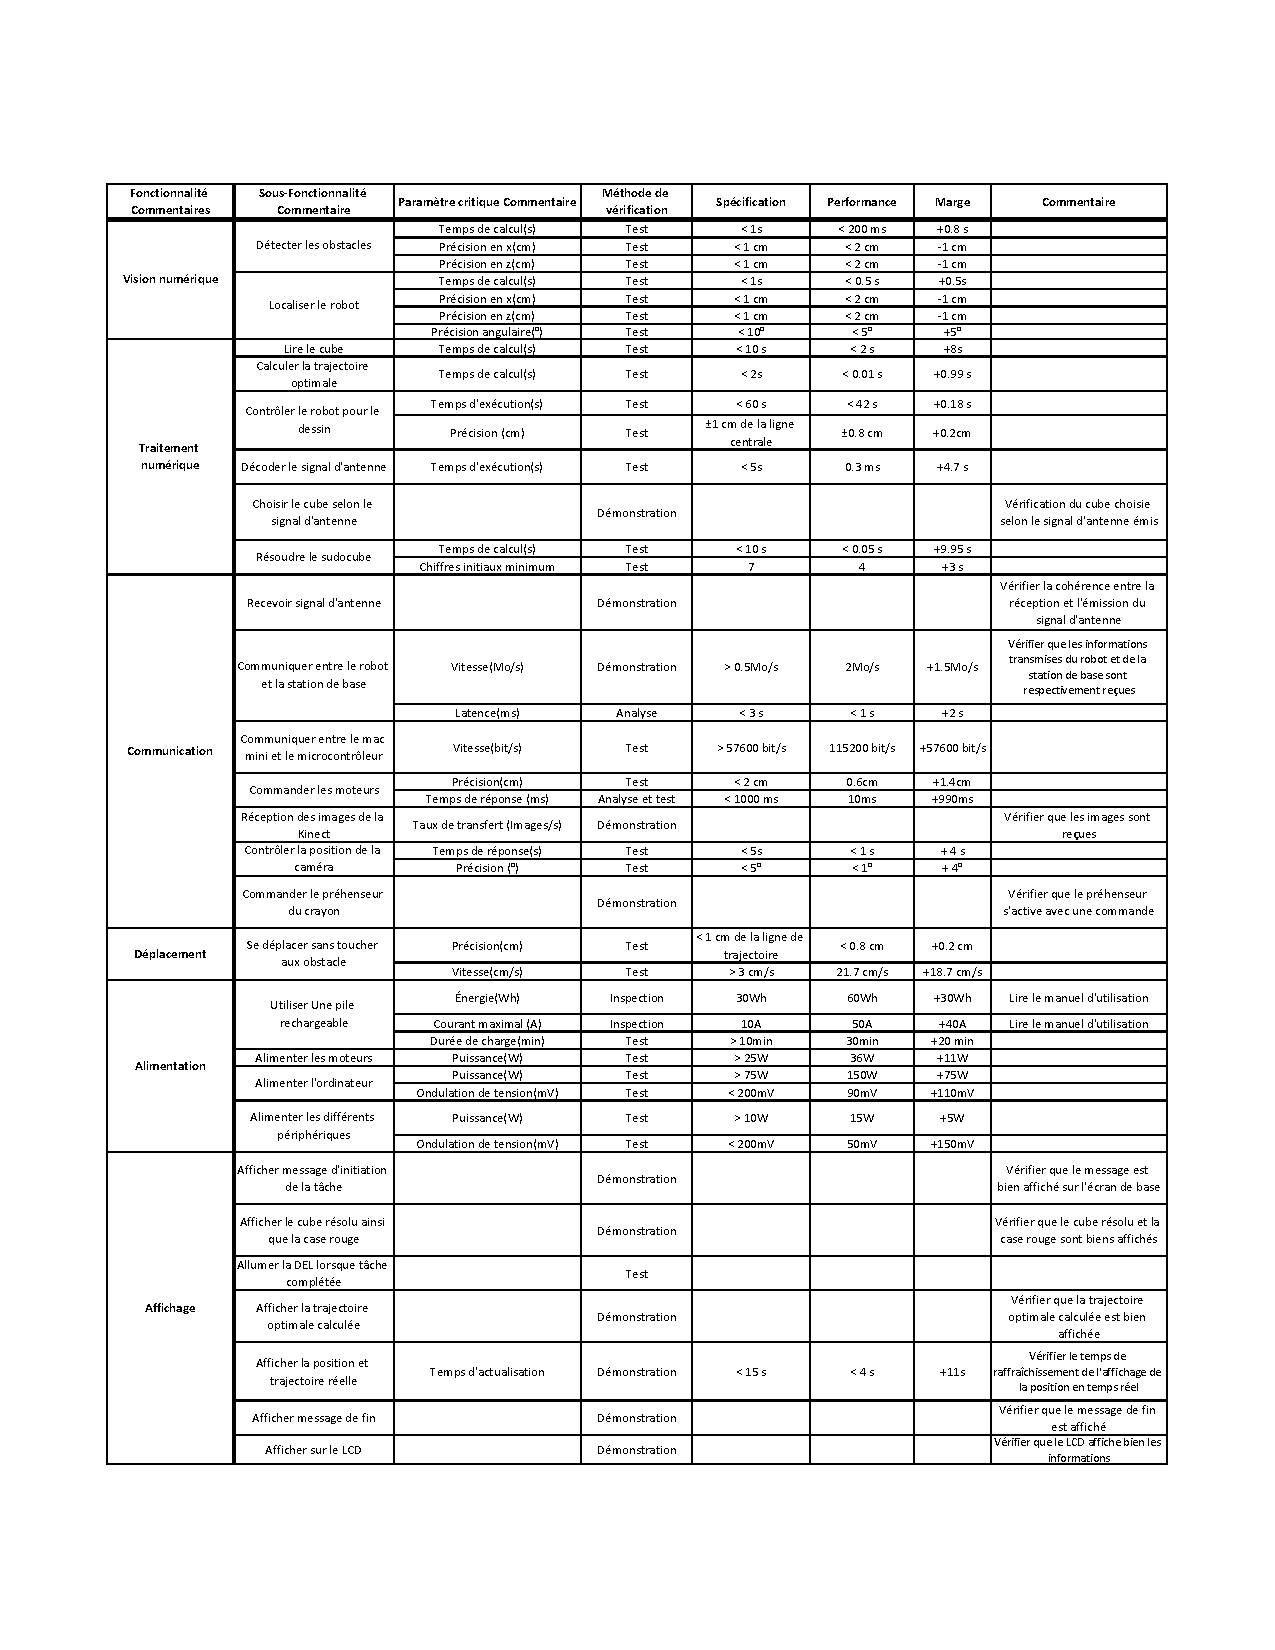
\includepdf[pages={-}]{tab_perf.pdf}
%\caption{Matrice de vérification des performances}
%\label{fig:diagSeq1Ite1} 
%\end{figure}
%

%!TEX root = ../rapport.tex
%!TEX encoding = UTF-8 Unicode

% Chapitres "Introduction"

% modifié par Francis Valois, Université Laval
% 31/01/2011 - version 1.0 - Création du document

\chapter{Vision 2$^e$ itération}
\label{vision2}

\section{Localisation avec la caméra embarquée}

La localisation avec la caméra embarquée est un système de localisation d'appoint dans le projet Kinocto. La classe Localisation doit recevoir une image et une orientation grossière selon le nord, sud, est ou ouest par rapport à la table. Elle doit ensuite être initialisée en fournissant un fichier .xml contenant les paramètres de calibration. Ces paramètres comprennent les paramètres intrinsèques de la caméra obtenus lors de la calibration, les paramètres liés à la distorsion de l'image par la lentille, les paramètres extrinsèques qui permettent de lier les points des images prises par la caméra à leur position par rapport à un système de référence virtuel ainsi que les paramètres qui permettent de recadrer ces coordonnées par rapport au centre du robot.

Avec l'image et les paramètres provenant de la calibration, les méthodes de localisation, de détermination de l'orientation et de mesure de l'angle par rapport au mur peuvent être utilisées.

\subsection{Localisation}

\subsubsection{Transformations}

Pour effectuer la localisation du robot, il faut trouver dans l'image reçue au moins deux points identifiables dont les coordonnées par rapport à la table sont connues. Dans le projet Kinocto, ces points incluent les coins de la table, les coins inférieurs des blocs de couleur, les coins du carré vert dessiné sur la table. Pour passer du système de coordonnées du robot à celui de la table, il faut résoudre le système d'équations suivant, où les points $P_1A$ et $P2_A$ sont les points dans le système de la table, $P_1R$ et $P_2R$ sont les mêmes points dans le système du robot et $t_X$ et $t_Y$ sont les coordonnées du robot dans le système de la table:

\begin{equation}
\label{eq1}
X_{1A} = X_{1R}cos(\theta) - Y_{1R}sin(\theta) + t_X
\end{equation}
\begin{equation}
\label{eq2}
Y_{1A} = X_{1R}sin(\theta) + Y_{1R}cos(\theta) + t_Y
\end{equation}
\begin{equation}
\label{eq3}
X_{2A} = X_{2R}cos{\theta} - Y_{2R}sin(\theta) + t_X
\end{equation}
\begin{equation}
\label{eq4}
Y_{2A} = X_{2R}sin(\theta) + Y_{2R}cos(\theta) + t_Y
\end{equation}

En soustrayant l'équation~\ref{eq3} de l'équation~\ref{eq1} ainsi que l'équation~\ref{eq4} de l'équation~\ref{eq2}, on élimine $t_X$ et $t_Y$ et on se retrouve avec deux équations que l'on peut combiner pour obtenir une équation à une inconnue, $\theta$. Il s'agit d'une équation de la forme $a cos(\theta) + b sin(\theta) = c$. Ce type d'équation peut être résolu en considérant la relation suivante:

\begin{equation}
a cos(\theta) + b sin(\theta) = R cos(\theta - \alpha)
\end{equation}

Où $R = \sqrt{a^2 + b^2}$ et $tan(\alpha) = \frac{b}{a}$. En isolant $\theta$, on obtient donc:

\begin{equation}
\theta = cos^{-1}(\frac{c}{\sqrt{a^2 + b^2}}) + tan^{-1}(\frac{b}{a})
\end{equation} 

Il suffit ensuite d'utiliser $\theta$ dans deux des équations initiales pour retrouver les coordonnées du robot selon le système de référence de la table $t_X$ et $t_Y$.

\subsubsection{Localisation des points}

\begin{enumerate}
\item{Coins de table}

Les points correspondant aux coins de table sont trouvés dans l'image en effectuant d'abord une segmentation sur le noir et en utilisant ensuite l'algorithme des lignes de Hough pour retrouver les lignes de bas de mur. L'intersection entre les lignes de bas de mur constitue le coin de la table. Un intérêt de cette méthode est qu'elle permet de retrouver les coins de table même lorsqu'un obstacle se trouve devant celui-ci.

\item{Coins du bas des blocs de couleur}

Les coins du bas des blocs de couleurs peuvent être retrouvés en trouvant les intersections entre les lignes de bas de mur et la ligne du bas du bloc de couleur, trouvée après segmentation sur le bleu et l'orange.

\item{Coins du carré vert}

Les coins internes du carré vert peuvent être retrouvés en segmentant sur le vert et en retrouvant les intersections entre les lignes avec la méthode décrite plus haut.
\end{enumerate}

\subsection{Orientation et angle par rapport au mur}

L'angle par rapport au mur peut être utile pour réorienter le robot pour la lecture des sudokus. Il est facilement obtenu en utilisant la ligne de bas de mur détectée précédemment. L'orientation peut être déduite en utilisant cet angle et l'orientation fournie à l'initialisation.

\subsection{Extraire les contours d'un sudocube}

La première étape d'extraction consiste à segmenter par couleur verte afin d'isoler le cadre du sudocube. Puis, un algorithme de détection des contours est appliqué pour trouver deux polygones rectangulaires. Ces polygones sont les bordures intérieures et extérieures du cadre. L'aire des rectangles est calculée pour vérifier que les polygones sont assez grands pour être ceux du cadre.

Ensuite, à partir du polygone intérieur du cadre on isole une sous-région de l'image principale. L'image obtenue est convertie en noir et blanc afin d'appliquer à nouveau un algorithme de contours afin de trouver les cases du sudocube. On sélectionne les polygones résultants selon leur aire. Si jamais le nombre de cases sélectionné n'est pas de 47, on recommence avec un seuil de tolérance différent pour l'algorithme de contour. Le polygone de la case rouge est obtenu en segmentant par couleur rouge et en appliquant à nouveau un algorithme de contour. 

Finalement, les images des cases sont triées en fonction de leur position en X et en Y dans l'image du sudocube et un algorithme de reconnaissance des caractères appliqué sur toutes les cases afin d'identifier les numéros. L'algorithme de reconnaissance utilise la technique KNearest. Les chiffres trouvés sont ajoutés dans la structure de données du sudocube et la position de la case rouge est spécifiée.

\section{Localisation avec la Kinect}

Pour aider au déplacement du robot, la Kinect a été utilisée afin de détecter la position des obstacles, la position du robot lui-même ainsi que sa position angulaire par rapport au point (0.0) de notre représentation cartésienne de la table. Toutefois, comme la Kinect est située à l'extérieur de la table de jeu, il faut une translation et une rotation des données obtenues afin de positionner les objets avec exactitude. Les 4 sections qui suivent expliquent en détail les différentes parties de l'algorithme de vision de la Kinect.

\subsection{Transformation des distances}
En premier lieu, il est important de clarifier quelles distances il est possible d'obtenir à l'aide de la Kinect. Le «Framework» OpenNI est capable de retourner 2 types de distances pour chacun des points dans l'image infrarouge obtenue de la Kinect. Le premier type de distances retourné est la longueur, en mètres, entre l'objectif et un point quelconque sur l'image. Le second type est dérivé du premier et correspond aux composantes X, Y et Z du vecteur de longueur entre l'objectif et la cible. Pour aider à la compréhension, les deux types de distances peuvent être représentés par les lignes vertes sur l'image \ref{fig:kinect_distance}. Toutefois, comme l'origine de notre représentation cartésienne de la table est située sur le coin inférieur droit de la table et que la Kinect n'est pas située à cet endroit, il est nécessaire d'obtenir la distance X et Y (lignes bleues sur l'image \ref{fig:kinect_distance}) entre l'origine et le point ciblé sur l'image obtenue de la Kinect. Pour y arriver, il suffit d'obtenir la position X et Y (lignes rouges sur l'image \ref{fig:kinect_distance}) de la lentille infrarouge de la Kinect ainsi que l'angle de la Kinect avec l'axe X de la table. Pour obtenir ces valeurs, nous utilisons une calibration simple présentée à la section \ref{s:kinectLocal}. Une fois la calibration effectuée, il est possible d'effectuer la transformation des distances de la Kinect vers les composantes X et Y recherchées à l'aide de règles de trigonométrie simples (Translation et Rotation). Toutefois, la Kinect possède une erreur de mesure qui augmente avec la distance. C'est pourquoi l'algorithme va toujours posséder une incertitude entre 1 et 3 cm pour chacun des points mesurés.

\begin{figure}[htbp]
\centering
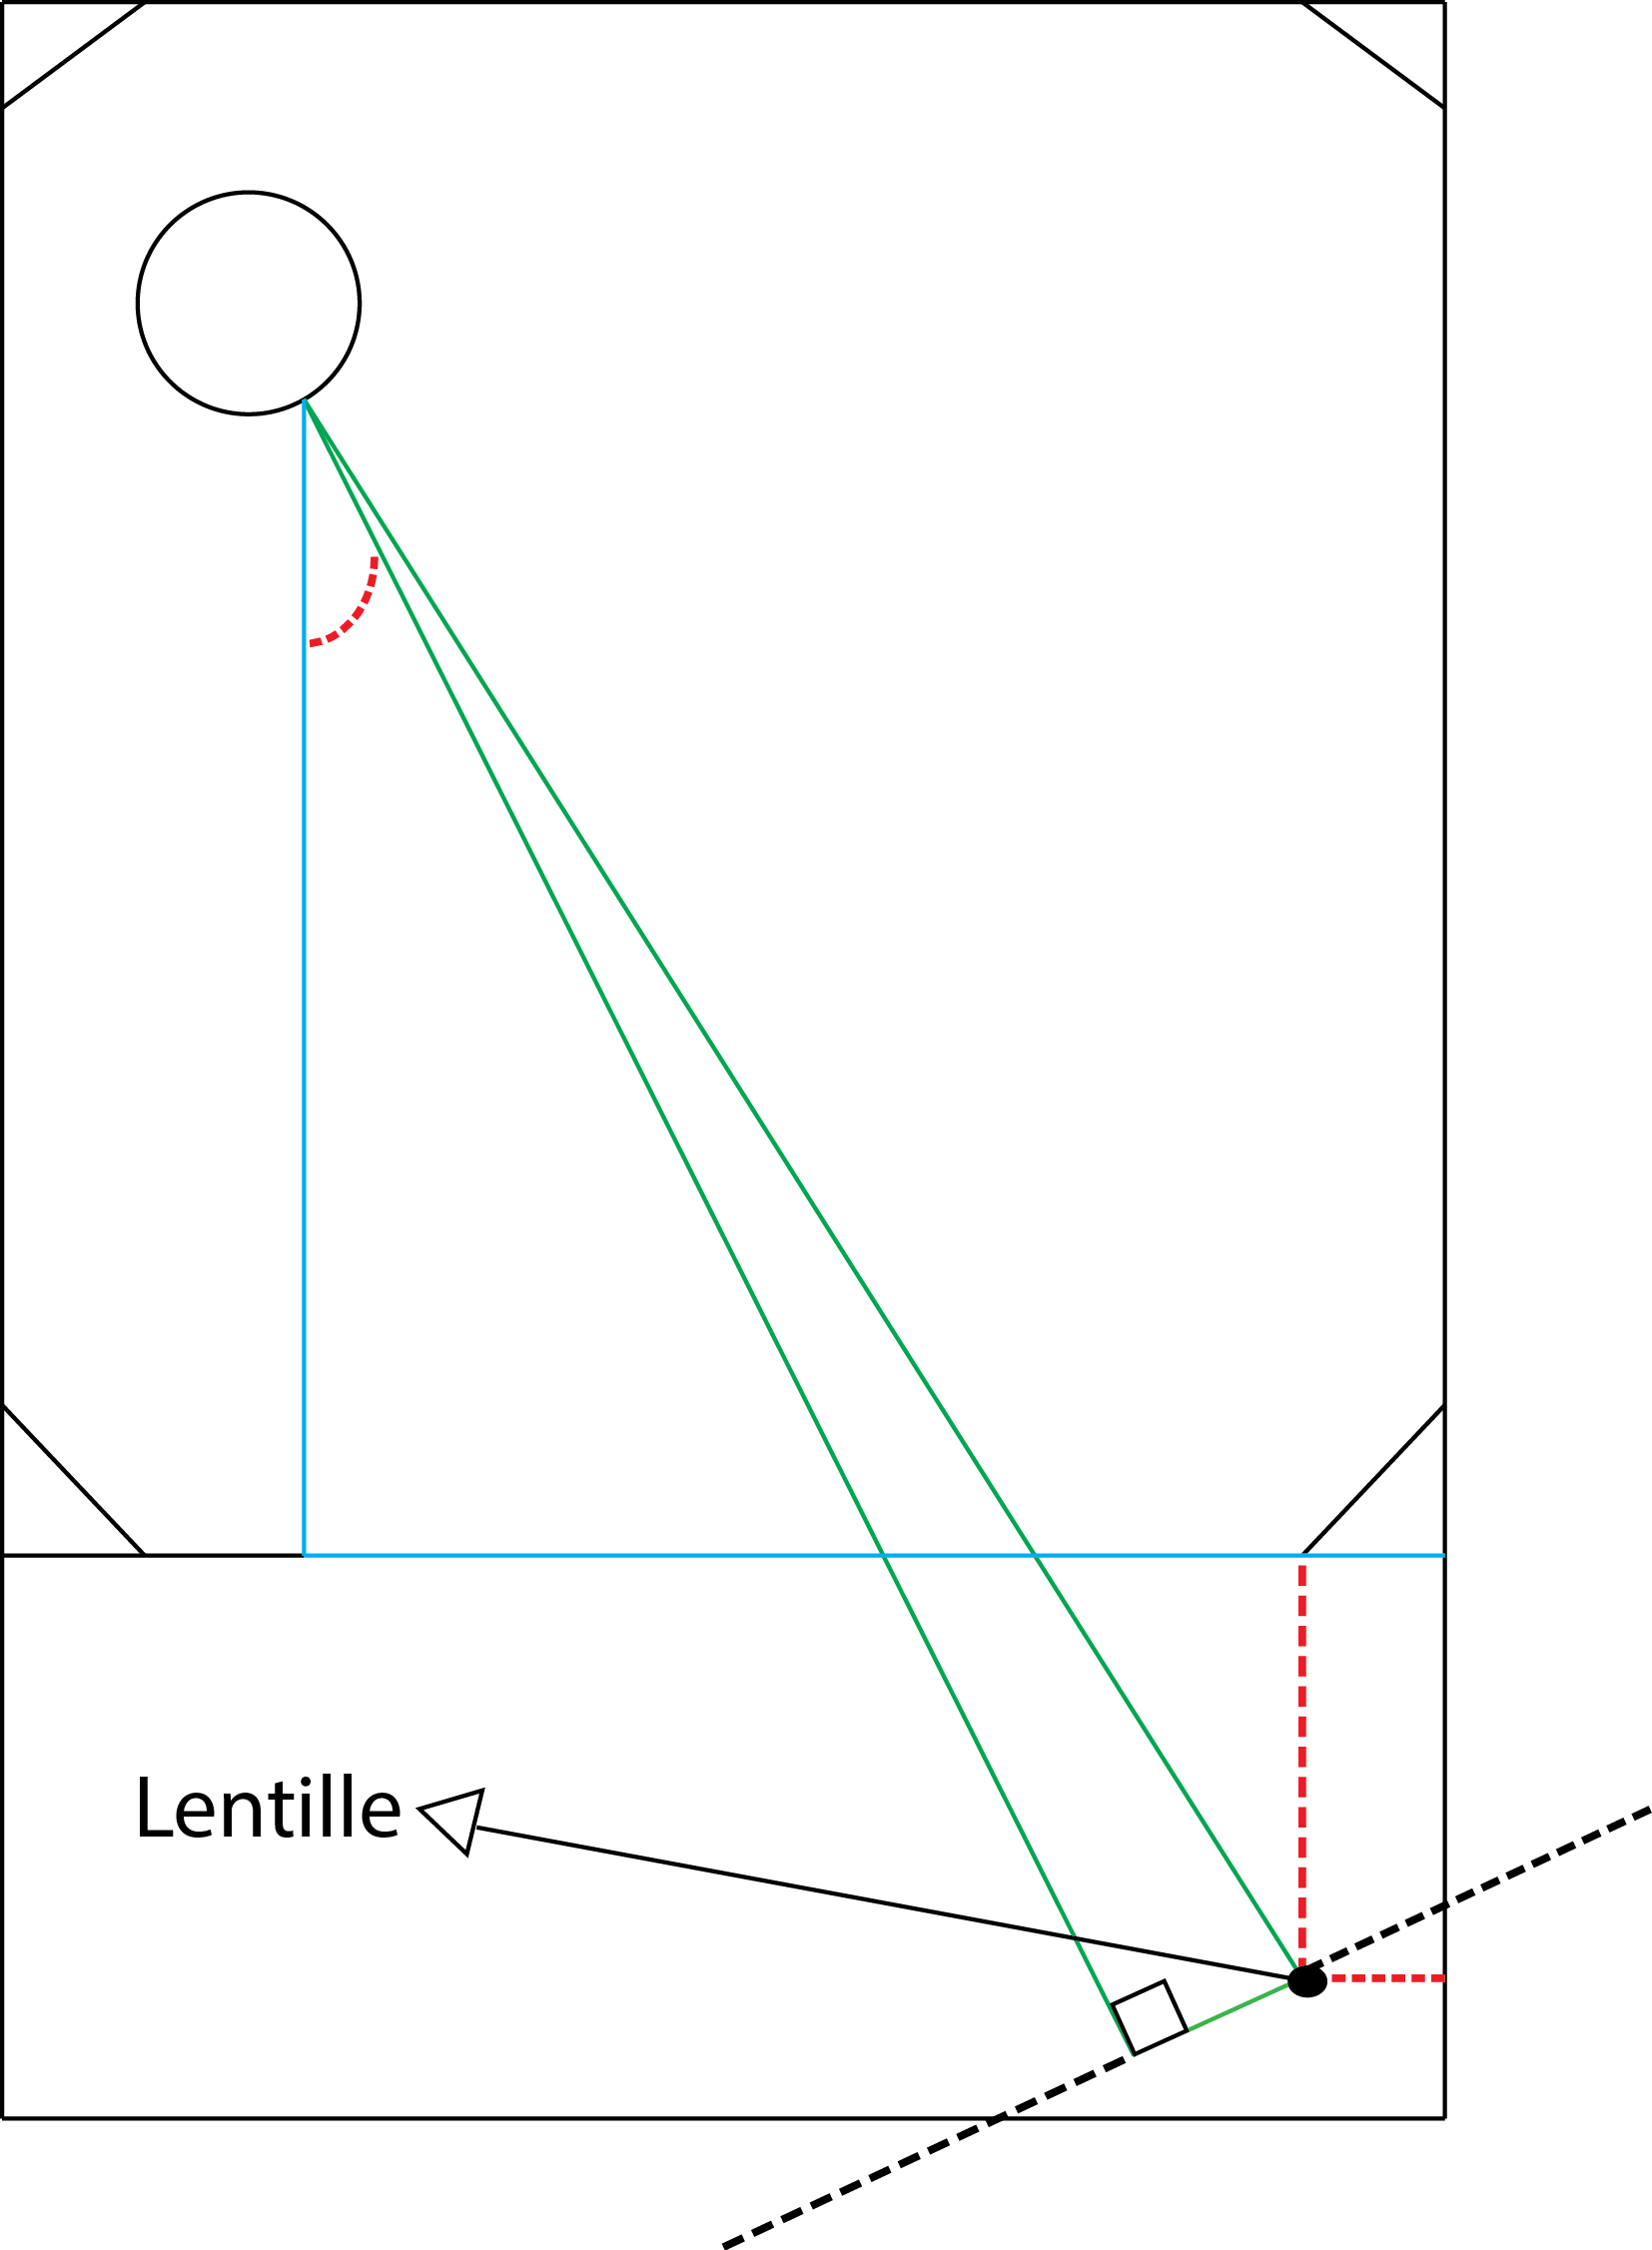
\includegraphics[scale=0.5]{fig/kinect_distance.png}
\caption{Schéma représentant la table et les différentes mesures obtenues avec la Kinect pour un point quelconque}
\label{fig:kinect_distance}
\end{figure}

\subsection{Localisation de la Kinect à l'aide de la calibration}
\label{s:kinectLocal}
Le but de la calibration est d'obtenir l'angle de la Kinect avec l'axe X de la table ainsi que la position de son objectif en XY par rapport au coin inférieur droit de la zone de jeu qui constitue notre point (0.0). Pour y arriver, un système, qui possède des dimensions connues, va positionner une plaque constituée d'un "Chessboard" sur la table à un endroit prédéterminé (ligne noire sur la table dans l'image \ref{fig:kinect_calibration}). Par la suite, une image RGB de la table est capturée à l'aide de la Kinect et les 2 points les plus éloignés horizontalement sur le "Chessboard" sont localisés. Ces 2 points sont reportés sur l'image de distances correspondante pour obtenir la distance XYZ de chacun des 2 points (lignes vertes sur l'image \ref{fig:kinect_calibration}). À l'aide de ces deux distances, les dimensions du petit triangle entre les deux points de la plaque de calibration sont trouvées (le triangle se situe en dessous de la plaque de calibration sur l'image \ref{fig:kinect_calibration}). En ayant les dimensions du triangle, il est possible de trouver l'angle de la Kinect, car celui-ci est le même que l'angle interne droit du triangle. Il suffit d'utiliser l'équation suivante avec les dimensions obtenues précédemment :

\begin{equation}
		Angle = \arctan \left( \frac{oppose}{adjacent} \right)
\end{equation}

\begin{figure}[htbp]
\centering
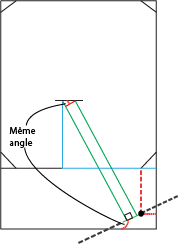
\includegraphics[scale=1]{fig/kinect_calibration.png}
\caption{Schéma représentant la table et les vecteurs nécessaires à la mesure de l'angle de la Kinect}
\label{fig:kinect_calibration}
\end{figure}

Pour obtenir la position de la Kinect, il est nécessaire de connaître la position réelle, par rapport au point (0.0), des 2 points utilisés pour la mesure de l'angle. En effectuant la rotation des distances de chacun, des points donnés par la Kinect pour ramener les mesures dans le plan XY de la table, les distances XY entre les points et l'objectif sont obtenues (lignes rouges pleines sur l'image \ref{fig:kinect_position}). En soustrayant les distances précédemment obtenues aux distances réelles mesurées (lignes bleues sur l'image \ref{fig:kinect_position}), la position de la Kinect est obtenue (lignes rouges pointillées sur l'image \ref{fig:kinect_position}).

\begin{figure}[htbp]
\centering
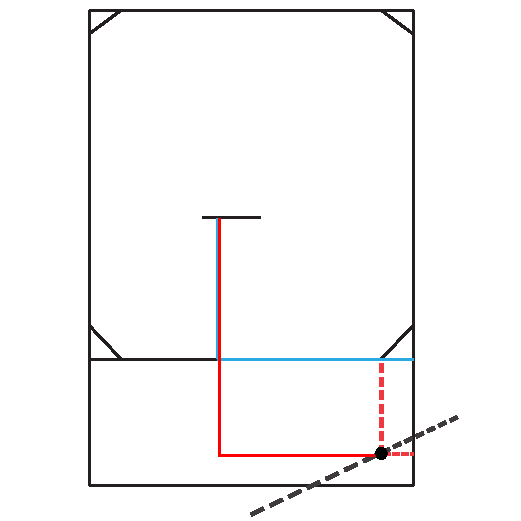
\includegraphics[scale=1]{fig/kinect_position.pdf}
\caption{Schéma représentant la table et les vecteurs nécessaires à la localisation de la Kinect}
\label{fig:kinect_position}
\end{figure}

\subsection{Détection des obstacles}
Comme il est possible d'obtenir n'importe quelle distance entre l'origine et un point quelconque sur l'image, un algorithme de recherche d'obstacles a été créé. Sachant que les obstacles sont situés dans une zone précise sur la table et que ceux-ci font 40cm de hauteur, il suffit de rechercher tout objet de cette hauteur situé dans la zone prédéfinie. La Kinect retourne la hauteur de chacun des points sur l'image infrarouge et permet de localiser les obstacles. De plus, à l'aide de calculs statistiques, l'algorithme est en mesure de trouver les obstacles lorsqu'ils sont presque alignés ou obstrués par un autre objet comme le robot. Comme cet algorithme dépend entièrement de l'algorithme de transformation des distances, les positions obtenues pour chacun des obstacles possèdent la même incertitude de 1 à 3 cm sur chaque mesure de distance effectuée. Pour améliorer la validité des mesures obtenues, une moyenne sur 3 images de distance est effectuée. En ce qui concerne l'efficacité de l'algorithme, différents tests montrent un temps de calcul d'environ 30 ms sur un Core 2 Duo 2.4 GHz pour obtenir la position du centre des deux obstacles.

\subsection{Détection du robot}
En ce qui concerne la détection du robot, un algorithme semblable à la détection des obstacles a été utilisé. Comme le robot possède une hauteur d'environs 20cm et une profondeur semblable, il est possible d'isoler, dans la matrice de distance, un carré qui correspond aux dimensions du robot. En plus de cette méthode, 2 "Chessboard" de couleurs différentes sont placés sur 2 faces opposées du robot. En recherchant les carrés sur le robot, il est possible de déterminer sa position comme l'algorithme précédant, mais en plus d'obtenir son angle, car la distance entre les points est connue ainsi que son orientation, car les "Chessboard" ne sont pas de la même couleur. Pour contrer l'erreur de position causée par la Kinect, la méthode de moyenne des distances utilisée pour la détection des obstacles est aussi appliquée à la détection du robot. Le temps de calcul est un peu plus élevé que la détection du robot et se situe aux alentours de 50 à 60 ms. 

%!TEX root = ../rapport.tex
%!TEX encoding = UTF-8 Unicode

% Chapitres "Introduction"

% modifié par Francis Valois, Université Laval
% 31/01/2011 - version 1.0 - Création du document

\chapter{Schémas électroniques 2$^{e}$ itération}
\label{electronics}
Le modèle de microcontrôleur employé est un Stellaris LM3S9B92. Les différentes entrées et sorties ont été fixées sur un circuit imprimé (PCB) dont le schéma est présenté à la figure \ref{fig:plan_micro}. 
\paragraph{}Tous les circuits électriques sont placés derrière un circuit de protection utilisant des fusibles dont le schéma est présenté à la figure \ref{fig:protection}. Ce circuit est prévu pour limiter les dégâts lors d'erreurs de manipulation ou de défectuosités électroniques. Par ailleurs, ces circuits sont actionnables par des interrupteurs placés devant les circuits respectifs. 
\paragraph{}L'alimentation 5V des périphériques est réalisée au moyen d'un circuit Buck 5V, le schéma est présenté à la figure \ref{fig:alim5V}.
\paragraph{}L'alimentation 24V du préhenseur et du Mac mini est réalisée au moyen d'un circuit Boost acheté chez un détaillant, pour lequel on ne dispose pas du plan de circuit en raison du secret d'ingénierie du fournisseur. La tension de sortie est variable avec un potentiomètre. La tension d'entrée est directement celle de la batterie. Une photo du dispositif est disponible à la figure \ref{fig:alim24Vphoto}.
\paragraph{}Le circuit de démodulation du signal Manchester émis sur les tables est réalisé au moyen du circuit présenté à la figure \ref{fig:manchester}. La clef de ce circuit est le LM567 qui est un circuit intégré permettant de syntoniser le signal d'antenne selon une largeur de bande que l'on établit au moyen des capacités présentes sur les différentes pines du LM567. Le LM567 permet d'isoler directement l'enveloppe du signal. Un comparateur à hystérésis est placé à la sortie du LM567 de manière à rendre plus uniformes et abruptes les transitions dans le signal d'enveloppe. 
\paragraph{}Le circuit de commande du préhenseur est présenté à la figure \ref{fig:prehenseur}. Il n'est composé que d'un transistor Mosfet qui permet d'activer la conduction du préhenseur (avec un courant proche de 150mA), directement à partir du microcontrôleur. Une diode de roue libre permet de décharger l'énergie de la bobine (préhenseur) lors des transitions.
\paragraph{}Le circuit de commande de la DEL est présenté à la figure \ref{fig:del_verte}. Il n'est composé que d'un transistor Mosfet qui permet d'activer la conduction de la DEL, une résistance de 100$\Omega$ permet de limiter le courant dans la DEL.

\begin{figure}
\centering
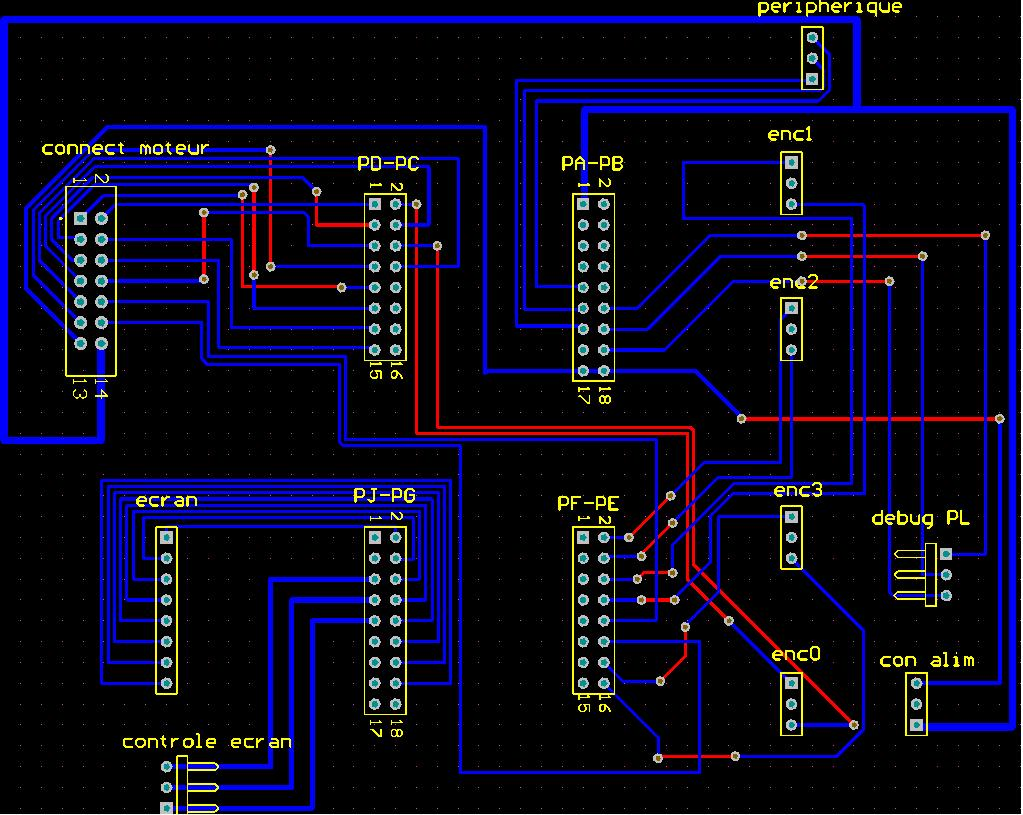
\includegraphics[scale=0.5]{fig/plan_micro.jpg}
\caption{Figure présentant le plan de l'alimentation 5V pour les périphériques}
\label{fig:plan_micro}
\end{figure}

\begin{figure}
\centering
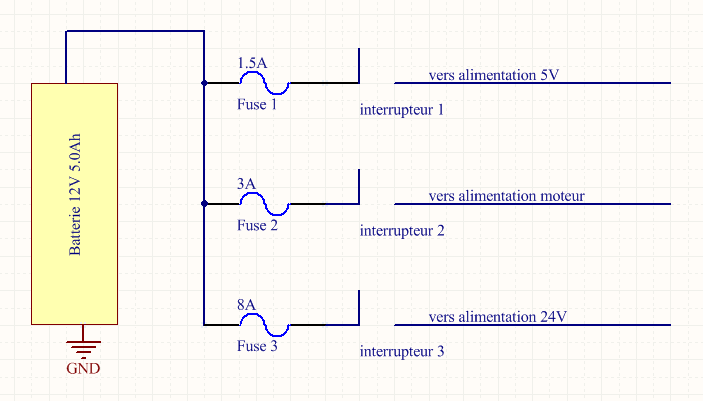
\includegraphics[scale=0.5]{fig/plan_circuit_protection.png}
\caption{Figure présentant le circuit de protection des circuits électriques}
\label{fig:protection}
\end{figure}

\begin{figure}[htbp]
\centering
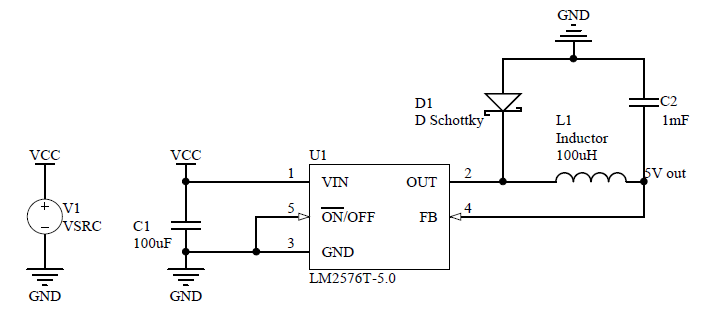
\includegraphics[scale=0.5]{fig/alim_5V.png}
\caption{Figure présentant le plan de l'alimentation 5V pour les périphériques}
\label{fig:alim5V}
\end{figure}

\begin{figure}[htbp]
\centering
\includegraphics[scale=0.1]{fig/alim_24V_photo.png}
\caption{Figure présentant une photo de l'alimentation 24V achetée telle quelle}
\label{fig:alim24Vphoto}
\end{figure}

\begin{figure}[htbp]
\centering
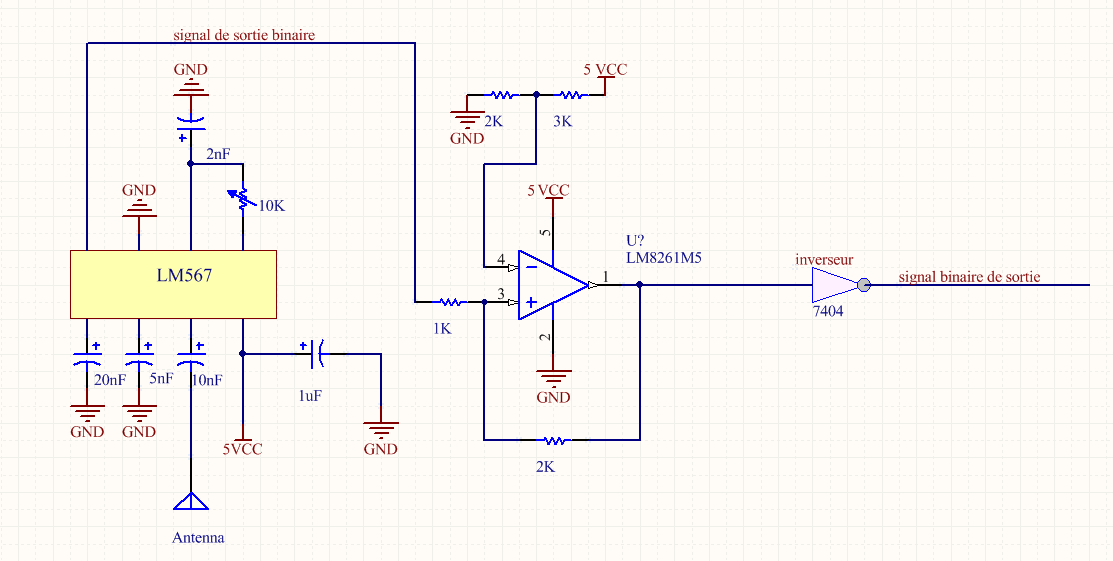
\includegraphics[scale=0.5]{fig/plan_manchester.png}
\caption{Figure présentant le plan du récepteur Manchester}
\label{fig:manchester}
\end{figure}

\begin{figure}[htbp]
\centering
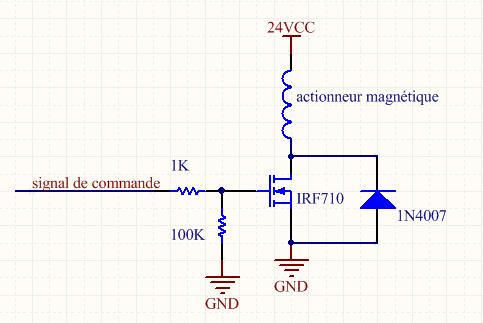
\includegraphics[scale=0.5]{fig/prehenseur.jpg}
\caption{Figure présentant le plan du circuit de commande du préhenseur}
\label{fig:prehenseur}
\end{figure}

\begin{figure}[htbp]
\centering
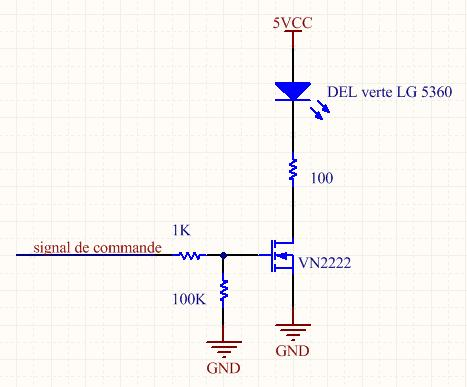
\includegraphics[scale=0.5]{fig/del_verte.jpg}
\caption{Figure présentant le plan du circuit de commande de la DEL verte}
\label{fig:del_verte}
\end{figure}
%!TEX root = ../rapport.tex
%!TEX encoding = UTF-8 Unicode

% Chapitres "Introduction"

% modifié par Francis Valois, Université Laval
% 31/01/2011 - version 1.0 - Création du document
\chapter{Post-mortem}

\section{Vision}

\subsection{Orientation avec la caméra embarquée}

L'utilisation de la matrice de transformation pour la localisation exige une matrice extrinsèque la plus parfaite possible. Avec plus de temps, il aurait peut-être été possible d'obtenir une bonne matrice et de la tester adéquatement. Il existe aussi une fonction dans opencv, reprojectImageTo3D pour la localisation des objets dans un espace 3D avec deux images prises avec deux caméras ou deux angles différents qui auraient pu être utilisées avec plus de temps et une calibration adéquate. 

Une autre méthode qui aurait pu être envisagée est une look-up table constituée en prenant une image d'une grille avec correspondance entre des points dont les coordonnées par rapport au robot sont connues. La transformation de la position du pixel dans l'image vers leurs coordonnées par rapport au robot aurait été faite en localisant les valeurs auxquelles elles correspondent dans la table et en effectuant une interpolation linéaire. Cette méthode aurait eu l'avantage d'être plus facilement et plus intuitivement testable que celles utilisant des matrices.

La localisation avec la caméra embarquée aurait potentiellement été plus précise que celle avec la Kinect, et particulièrement d'obtenir la position du robot lorsqu'il n'est pas possible de le faire avec la Kinect, ce qui survient surtout dans les positions les plus éloignées. 

La fiabilité de la méthode de localisation des points à l'intersection des Hough lines aurait également dû être améliorée pour pouvoir l'utiliser dans un algorithme de localisation. En ajustant la saturation des images prises et la segmentation, il était possible d'avoir la position des coins inférieurs des blocs de couleur dans la plupart des cas, mais il arrivait souvent que le positionnement s'écarte beaucoup de la position réelle à cause de l'erreur sur les droites retenues.


\subsection{Vision par Kinect}
La vision à l'aide de la Kinect a été une des parties les plus ardues tout au long du projet. Sachant que la technologie est relativement nouvelle, la documentation à son sujet est très restreinte et souvent incomplète. Il a donc fallu effectuer plusieurs tests et développer nos propres algorithmes pour arriver à quelque chose de fonctionnel. De plus, les frameworks ne semblent pas encore tout à fait matures pour en faire une utilisation simple. Nous avons qu'à penser à la distorsion de la caméra infrarouge qui a causé d'énorme problème lors des tests de nos algorithmes de transformation de distances. Cette distorsion pourrait être simplement corrigée au travers du framework et la documentation pourrait en faire mention. Une autre idée possible pour améliorer la précision est l'utilisation d'une lookup table de correction en XZ. En effectuant la même méthodologie que pour la courbe de correction en X présenté à la section \ref{s:distortion}, mais à plus grande échelle, soit plus de 50 points partout sur la table, il serait possible d'obtenir une très bonne correction.

Toutefois, outre le problème majeur de distorsion, la Kinect permet d'obtenir facilement la distance de tout objet dans son champ de vision avec une certaine précision. Ainsi, à l'aide d'algorithme de détection et de statistique, il a été fort simple d'obtenir la position en 3D des obstacles et du robot sur la table. Comme la Kinect effectue tout le traitement de conversion IR-Distance, nos algorithmes sont très efficaces en temps d'exécution. Ainsi, pour la détection des obstacles, l'algorithme prend entre 30 et 60 ms ce qui est très rapide pour une telle détection. Du côté de la détection du robot, il a été nécessaire d'utiliser la caméra RGB en plus de la caméra infrarouge, car le robot est presque aussi haut que les murs de la table. Ainsi, il devient ardu d'extraire le robot du nuage de point lorsque celui-ci est proche d'un mur ou bien des obstacles. La principale difficulté de l'utilisation de la caméra RGB est de savoir ce que nous devons ignorer et ce que nous devons garder. Dans la première version de la détection du cadre bleu sur le robot, dès que quelque chose de bleu entrait dans le champ de vision de la caméra, l'algorithme n'était plus apte à trouver la position du robot et retournait des valeurs aberrantes. Dans la deuxième version, chacune des zones bleues trouvées par l'algorithme est comparée aux distances de la Kinect. Ainsi, lorsque les zones bleues sont situées à l'extérieur de la table, il suffit de les ignorer. Cette composition IR-RGB est vraiment intéressante. Toutefois, en se servant de la caméra RGB, il faut ajouter un temps considérable de traitement pour trouver le cadre bleu ainsi que les différents petits carrés, car la détection n'est pas effectuée directement par la Kinect comme la conversion IR-Distance. Ce traitement de l'image ajoute environ 200ms de plus aux 30 à 60ms de détection de forme dans le nuage de point. Ce temps d'excution est toutefois en déca de la seconde et est donc extremement rapide et adapté à la mise à jour en temps réel de la position du robot.

En écartant la précision imparfaite de notre implantation qui ne demande qu'à être améliorée, le placement des cadres bleus oblige le robot à se placer d'une certaine façon pour que celui-ci soit détecté. Une amélioration possible aurait été de placer des carrés sur les faces non détectées pour permettre la détection à 360 degrés, mais il aurait été nécessaire de créer un algorithme de choix de carrés pour en choisir 1 seul, car dans la plupart des cas, deux carrés auraient été visibles.

\section{Déplacements}

Dans l'ensemble, le robot a un asservissement linéaire en vitesse qui dépasse largement les autres équipes en termes de temps de réponse et de stabilité directionnelle. La stratégie de déplacement aurait pu être optimisée avec l'utilisation des déplacements en diagonal. Comme l'asservissement était en vitesse, nous aurions eu à intégrer des plages de décélérations calibrées selon les plages d'asservissements. Afin d'assurer l'unicité de l'ensemble, d'autres calibres d'asservissements auraient dû être ajoutés. 

\section{Dessins}

Afin de compenser les disparités de constitutions des roues de notre robot, qui avaient énormément d'impact sur nos performances, un asservissement en position utilisant la vision aurait pu être implanté afin de compenser les erreurs. Pour se faire, nous aurions pu centrer le préhenseur et effectuer des rotations lors des croisements afin de toujours détecter le cadre vert. L'implantation de l'asservissement de déplacement pour les diagonales aurait pu être employé à cet effet, jumelé à la détection du cadre vert, qui aurait du être adaptée pour un robot qui se déplace. Évidemment, le temps requis de conception est particulièrement énorme et un tel ajustement aurait requis plusieurs semaines. 



\end{document}
% Fin du document

